\documentclass[11pt]{article}
\usepackage[margin=0.6in]{geometry}
\usepackage{amssymb, amsmath, amsfonts, amsthm}
\usepackage{mathpazo}
\usepackage{setspace}
\usepackage{fancyhdr}
\usepackage{enumerate}
\usepackage{tikz}
\usepackage{float}
\usetikzlibrary{automata,positioning}
\usepackage{fancybox, graphicx}


\pagestyle{fancyplain}
\lhead{\textbf{\NAME\ }}
\rhead{CPSC 313, \today}

\newcommand\question[2]{
\shadowbox{
\begin{minipage}{45em}\vspace{1ex}\textbf{Problem #1}
\newline
\vspace{1ex}
\end{minipage}
}
\vspace{1ex}
}

\begin{document}
\linespread{0.9}
\newcommand\NAME{Eddy Qiang}
\question{1}{John X and Jane Y}
\begin{enumerate}




%problem 1
Assume L\textsubscript{1} is regular for contradiction. Let p be the pumping length given by the pumping lemma. Let s = 5 + 5\textsuperscript{p} = 10, s $\in$ L\textsubscript{1} and $|$s$|$ = p+5 $>$ p, the pumping lemma guarantees that s can be divided into three pieces, s = xyz. By condition 3, we know $|$xy$|$ $\le$ p, so y has to take the form 5\textsuperscript{k} for some k
. By condition 1, for each i $\geq$ 0, xy\textsuperscript{i}z  $\in$ L\textsubscript{1}. Let i = 2, so we have xy\textsuperscript{2}z = xyyz. Observe that by pumping another y the string becomes 5 + 55 = 10 which is not in the language L\textsubscript{1}. Therefore we arrive at a contradiction and reject our initial assumption that L\textsubscript{1} is regular.

\end{enumerate}
\newpage

\question{2}{John X and Jane Y} % add your collaborators here.

% begin your solution here
\begin{enumerate}

%problem 2
\begin{align*} 
S& \rightarrow WT \\
W& \rightarrow b \text{ }|\text{ }\epsilon \\ 
T& \rightarrow VXXX  \\ 
V& \rightarrow XbXXXW \text{ }| \text{ }bXXXXW \text{ }|\text{ }\epsilon \\ 
W& \rightarrow XXXX \text{ }|\text{ } WW \text{ }|\text{ }\epsilon\\ 
X& \rightarrow a \text{ }|\text{ }b \\ 
\end{align*}


\end{enumerate}
\newpage

\question{3}{John X and Jane Y} % add your collaborators here.

% begin your solution here
\begin{enumerate}

\documentclass[12pt]{article}
\usepackage{tikz}

\begin{document}

\begin{center}
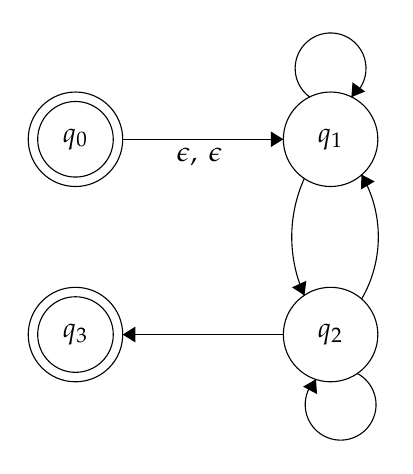
\begin{tikzpicture}[scale=0.2]
\tikzstyle{every node}+=[inner sep=0pt]
\draw [black] (27.9,-25.8) circle (3);
\draw (27.9,-25.8) node {$q_0$};
\draw [black] (27.9,-25.8) circle (2.4);
\draw [black] (44.1,-25.8) circle (3);
\draw (44.1,-25.8) node {$q_1$};
\draw [black] (44.1,-38.2) circle (3);
\draw (44.1,-38.2) node {$q_2$};
\draw [black] (27.9,-38.2) circle (3);
\draw (27.9,-38.2) node {$q_3$};
\draw [black] (27.9,-38.2) circle (2.4);
\draw [black] (30.9,-25.8) -- (41.1,-25.8);
\fill [black] (41.1,-25.8) -- (40.3,-25.3) -- (40.3,-26.3);
\draw (36,-26.3) node [below] {$\epsilon,\mbox{ }\epsilon\mbox{ }$};
\draw [black] (41.1,-38.2) -- (30.9,-38.2);
\fill [black] (30.9,-38.2) -- (31.7,-38.7) -- (31.7,-37.7);
\draw [black] (42.436,-35.721) arc (-155.64846:-204.35154:9.024);
\fill [black] (42.44,-35.72) -- (42.56,-34.79) -- (41.65,-35.2);
\draw [black] (46.063,-28.045) arc (30.22996:-30.22996:7.856);
\fill [black] (46.06,-28.04) -- (46.03,-28.99) -- (46.9,-28.48);
\draw [black] (42.777,-23.12) arc (234:-54:2.25);
\fill [black] (45.42,-23.12) -- (46.3,-22.77) -- (45.49,-22.18);
\draw [black] (45.788,-40.666) arc (62.1301:-225.8699:2.25);
\fill [black] (43.17,-41.04) -- (42.35,-41.51) -- (43.24,-41.98);
\end{tikzpicture}
\end{center}

\end{document}


%explanation
this pda

\end{enumerate}
\newpage

\question{4}{John X and Jane Y} % add your collaborators here.

% begin your solution here
\begin{enumerate}
\item Here is the solution for part 1.

L\textsubscript{2} will accept strings where the difference of the number of a's and b's is no greater than 2. So when you concatenate L\textsubscript{b} with it, the new language will contain at least 4 b's. The intersection between this and L\textsubscript{2} will have to contain the strings with at least 4 b's, so then there must be so there must be at least 2 a's as well to be a part of L\textsubscript{2}. Then lastly it is concatenated with L\textsubscript{a} which adds two more a's to it so now it will have at least four a's with a equal number of b's.
{

L = L\textsubscript{a}(L\textsubscript{2}L\textsubscript{b} \cap L\textsubscript{2}) = \{a\textsuperscript{i}b\textsuperscript{j} \  \vert \ i \geq 4 \ , \ j=i\}
\newline
}

\item Here is the solution for part 2.
\newline
This NFA will recognize strings that contain two 0's separated by a sub-string with a length that is a multiple of 3. The regular expression for this language is (0+1)*0((0+1)(0+1)(0+1))*0(0+1)*. 
\newline
\newline
The expression is correct because the expression starts and ends with (0+1)*0...*0(0+1)*, this part will require there be at least two 0's. The inside part ((0+1)(0+1)(0+1))* will require you to choose either a 0 or 1 three times, and since it is closed under *, the length can be any multiple of 3. Therefore this expression will recognize strings that contain two 0's separated by a sub-string with a length that is a multiple of 3.
\end{enumerate}
\newpage
\end{document}